\subsection{Wave number}
\label{datak}
Wave number is a measure of the number of waves per unit distance and is inversely proportional to wave speed. Hourly observations  using an Argus video monitoring system mounted on shore are available during October 2015. Photogrammetry is performed on the video to derive the dominant wave frequencies and wave numbers in the survey area \citep{holman2013}. Data is available for a 2D area at the FRF survey site. A 1D profile is extracted from the 2D data along a transect corresponding to the position of the model boundary point (\textit{y} = 950 m). Figure~\ref{k1Dmean} shows statistics for wave number, \textit{k}, along the 1D transect. Wave number is shown to be slightly more variable over time close to the coast. Mean wave number increases toward the shoreline, as expected.



\begin{figure}[H]
\centering
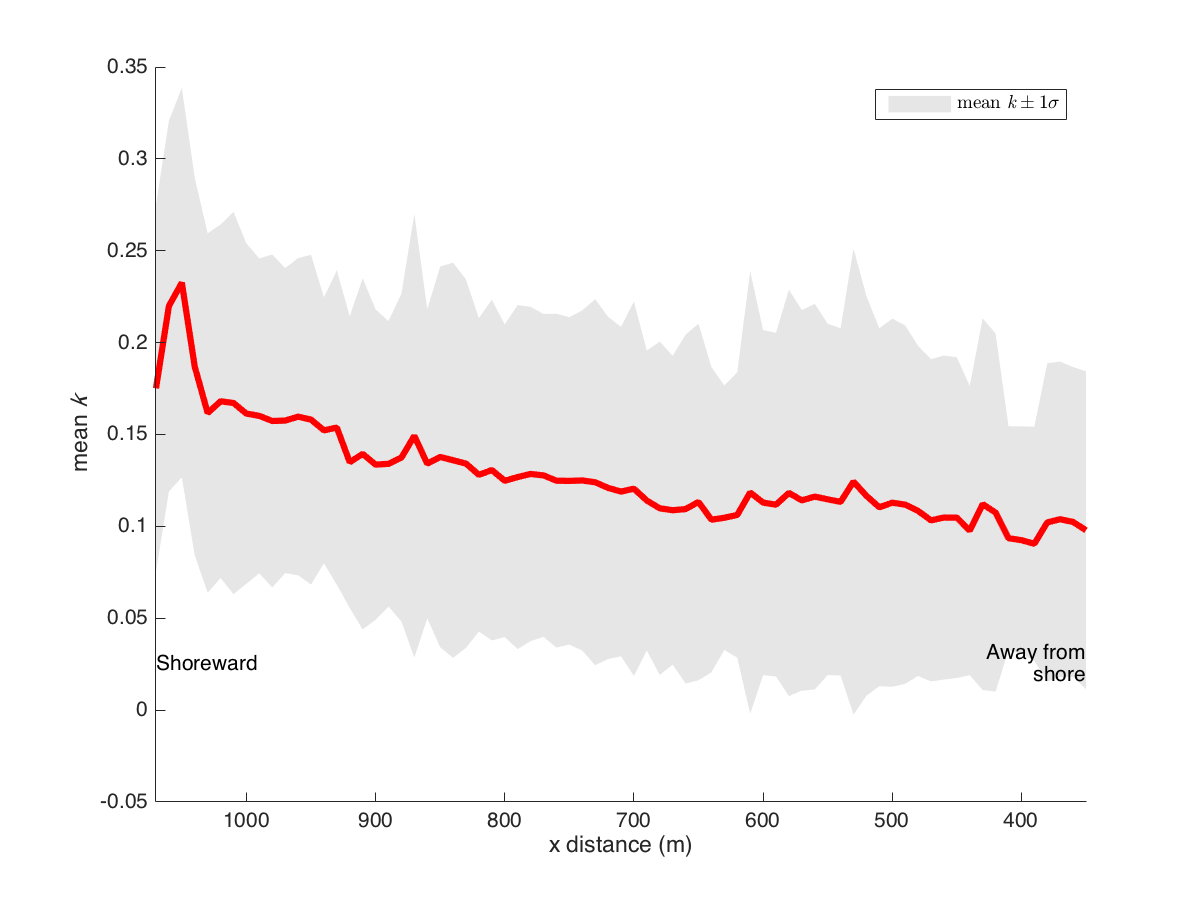
\includegraphics[width=.55\linewidth]{img/k1Dmean_std.png}
\caption{Wave number along the transect where the model boundary condition is located. Mean wave number, \textit{k}, during October 2015 is shown in red. Gray envelopes show $\pm$ 1$\sigma$ standard deviation in \textit{k}. Wave number is observed to be relatively larger and more variable closer to shore.}
\label{k1Dmean}
\end{figure}